Для создания панорамы использовались фотографии, приведенные на рисунке \ref{img:input_imgs}, а результат работы написанной программы приведен на рисунке \ref{img:result}.

\begin{figure}[h!]
	\center {
		\includegraphics[width=\linewidth / 2, angle = -90]{img/left} \vspace{5mm}
		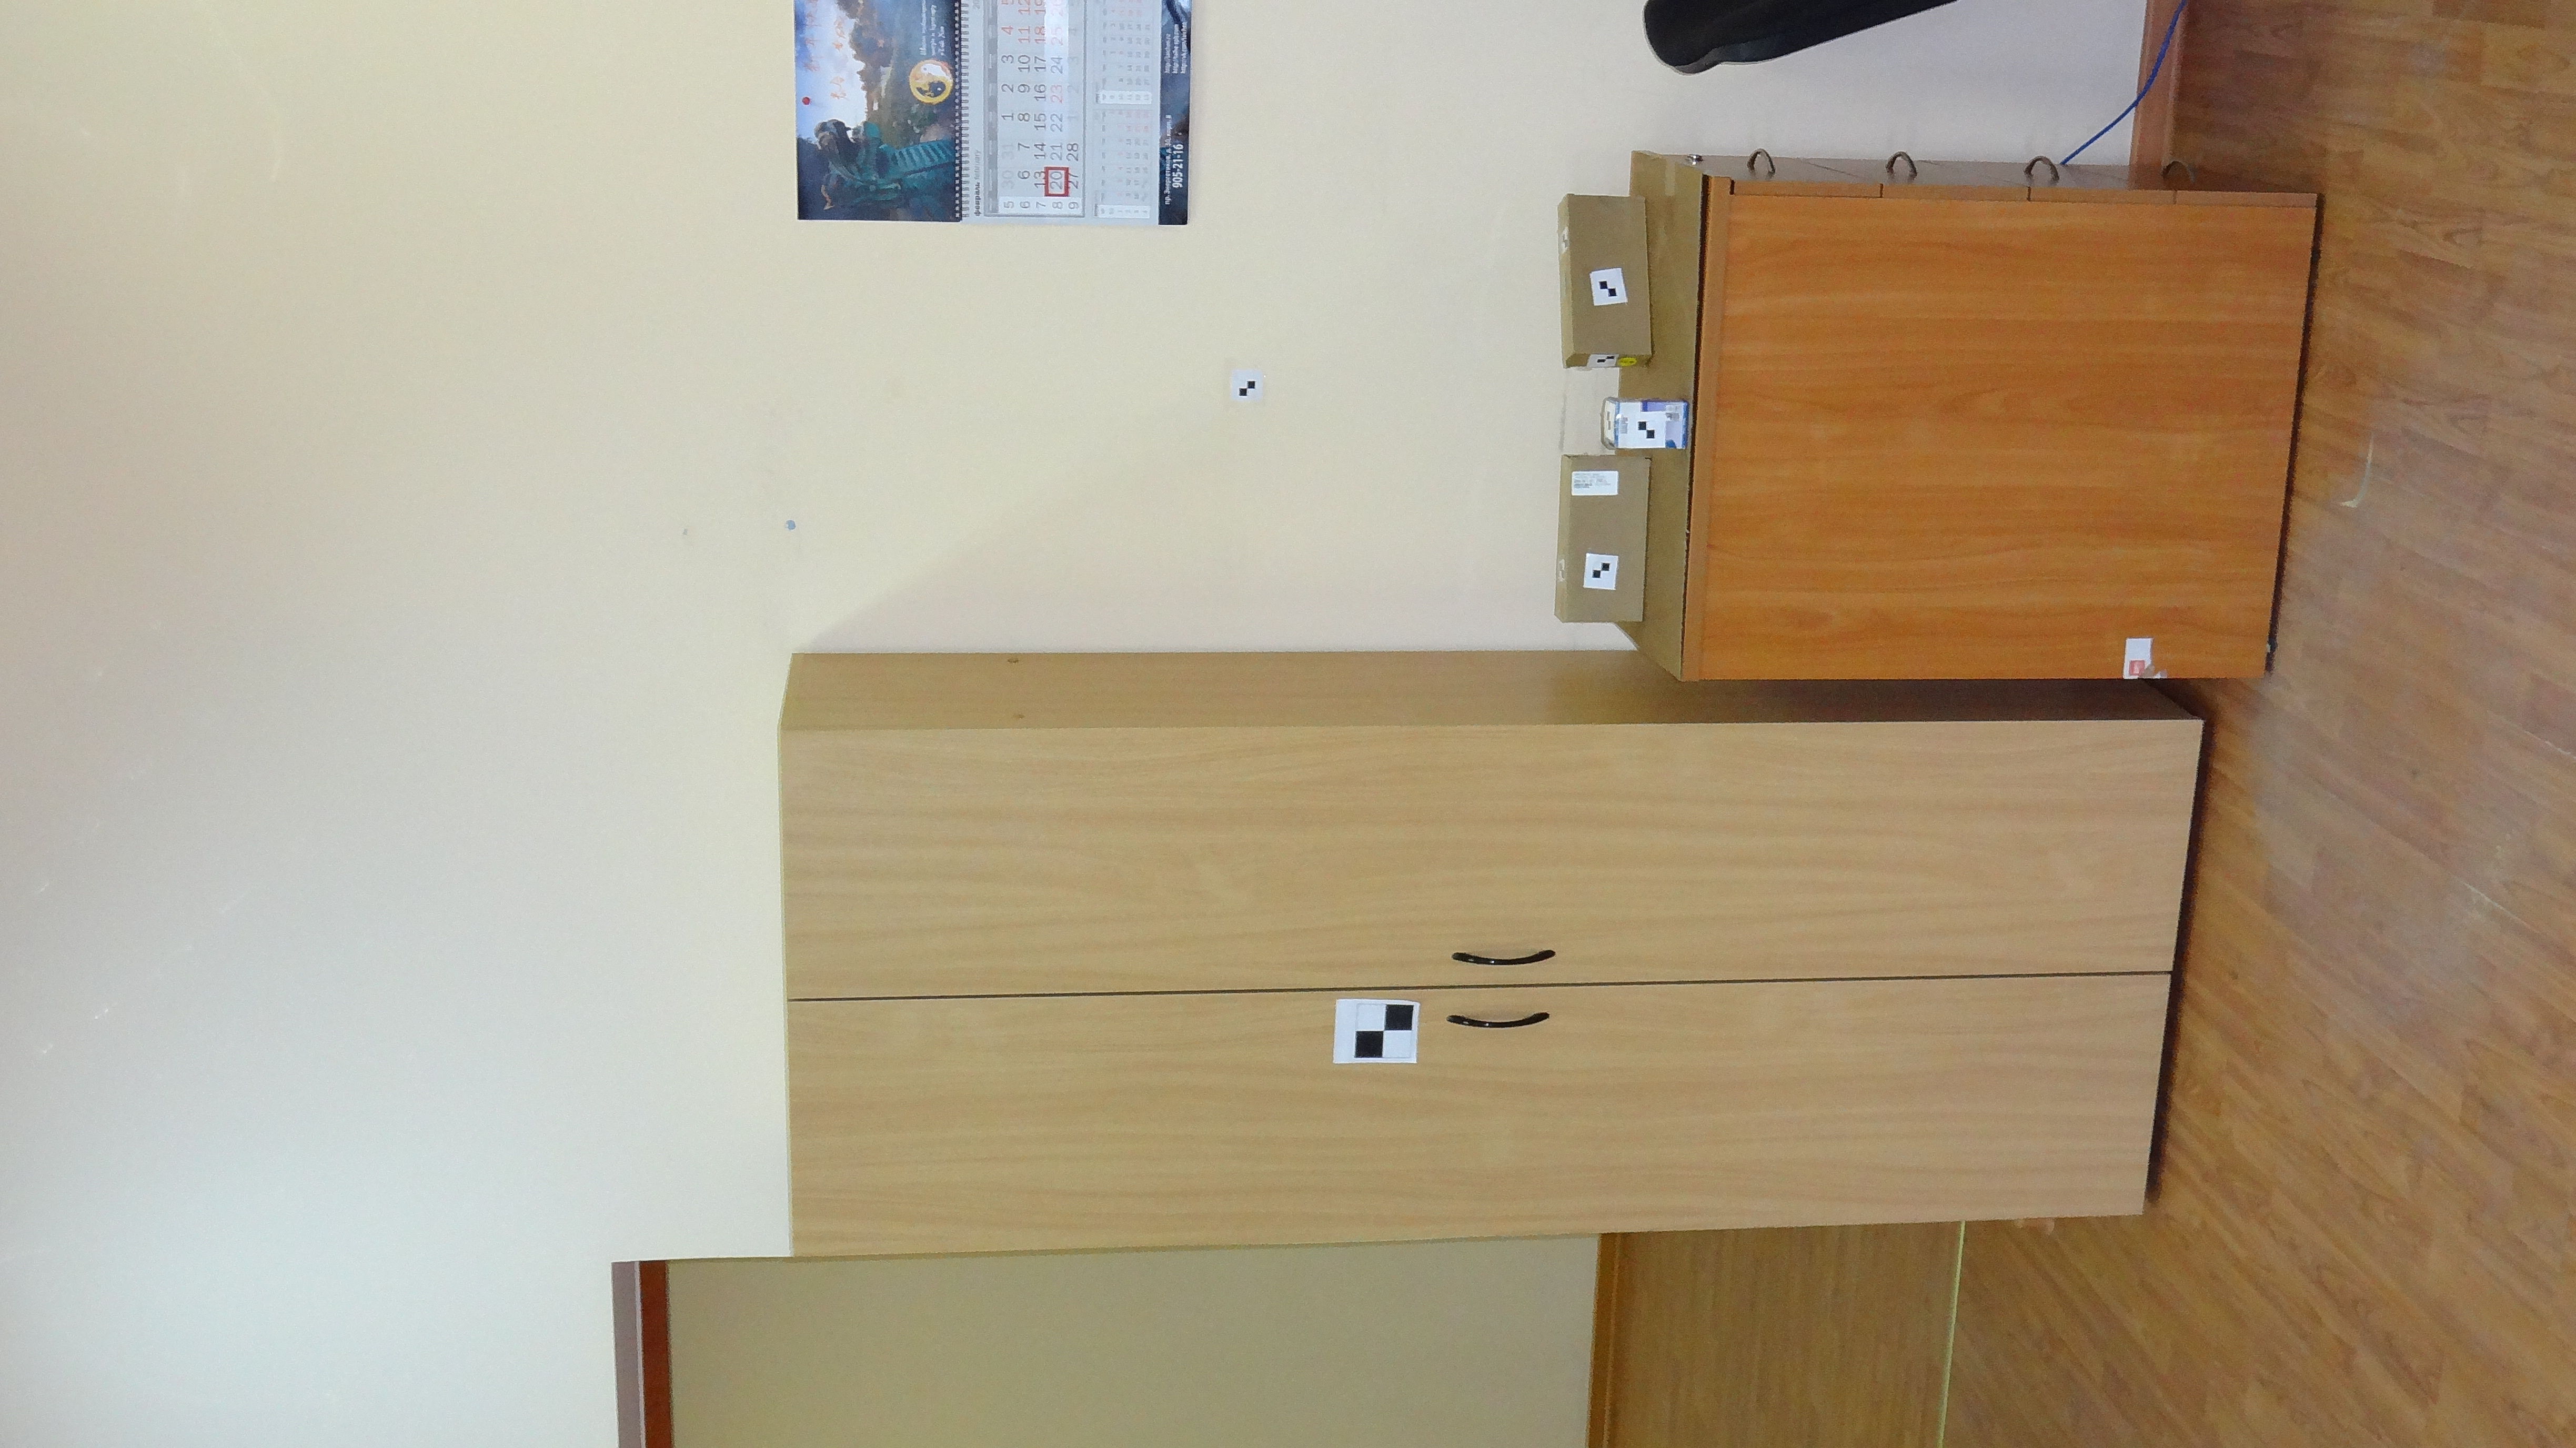
\includegraphics[width=\linewidth / 2, angle = -90]{img/right}
	}
	\caption{Фотографии для создания панорамы}
	\label{img:input_imgs}
\end{figure}

\begin{figure}[h!]
	\center {
		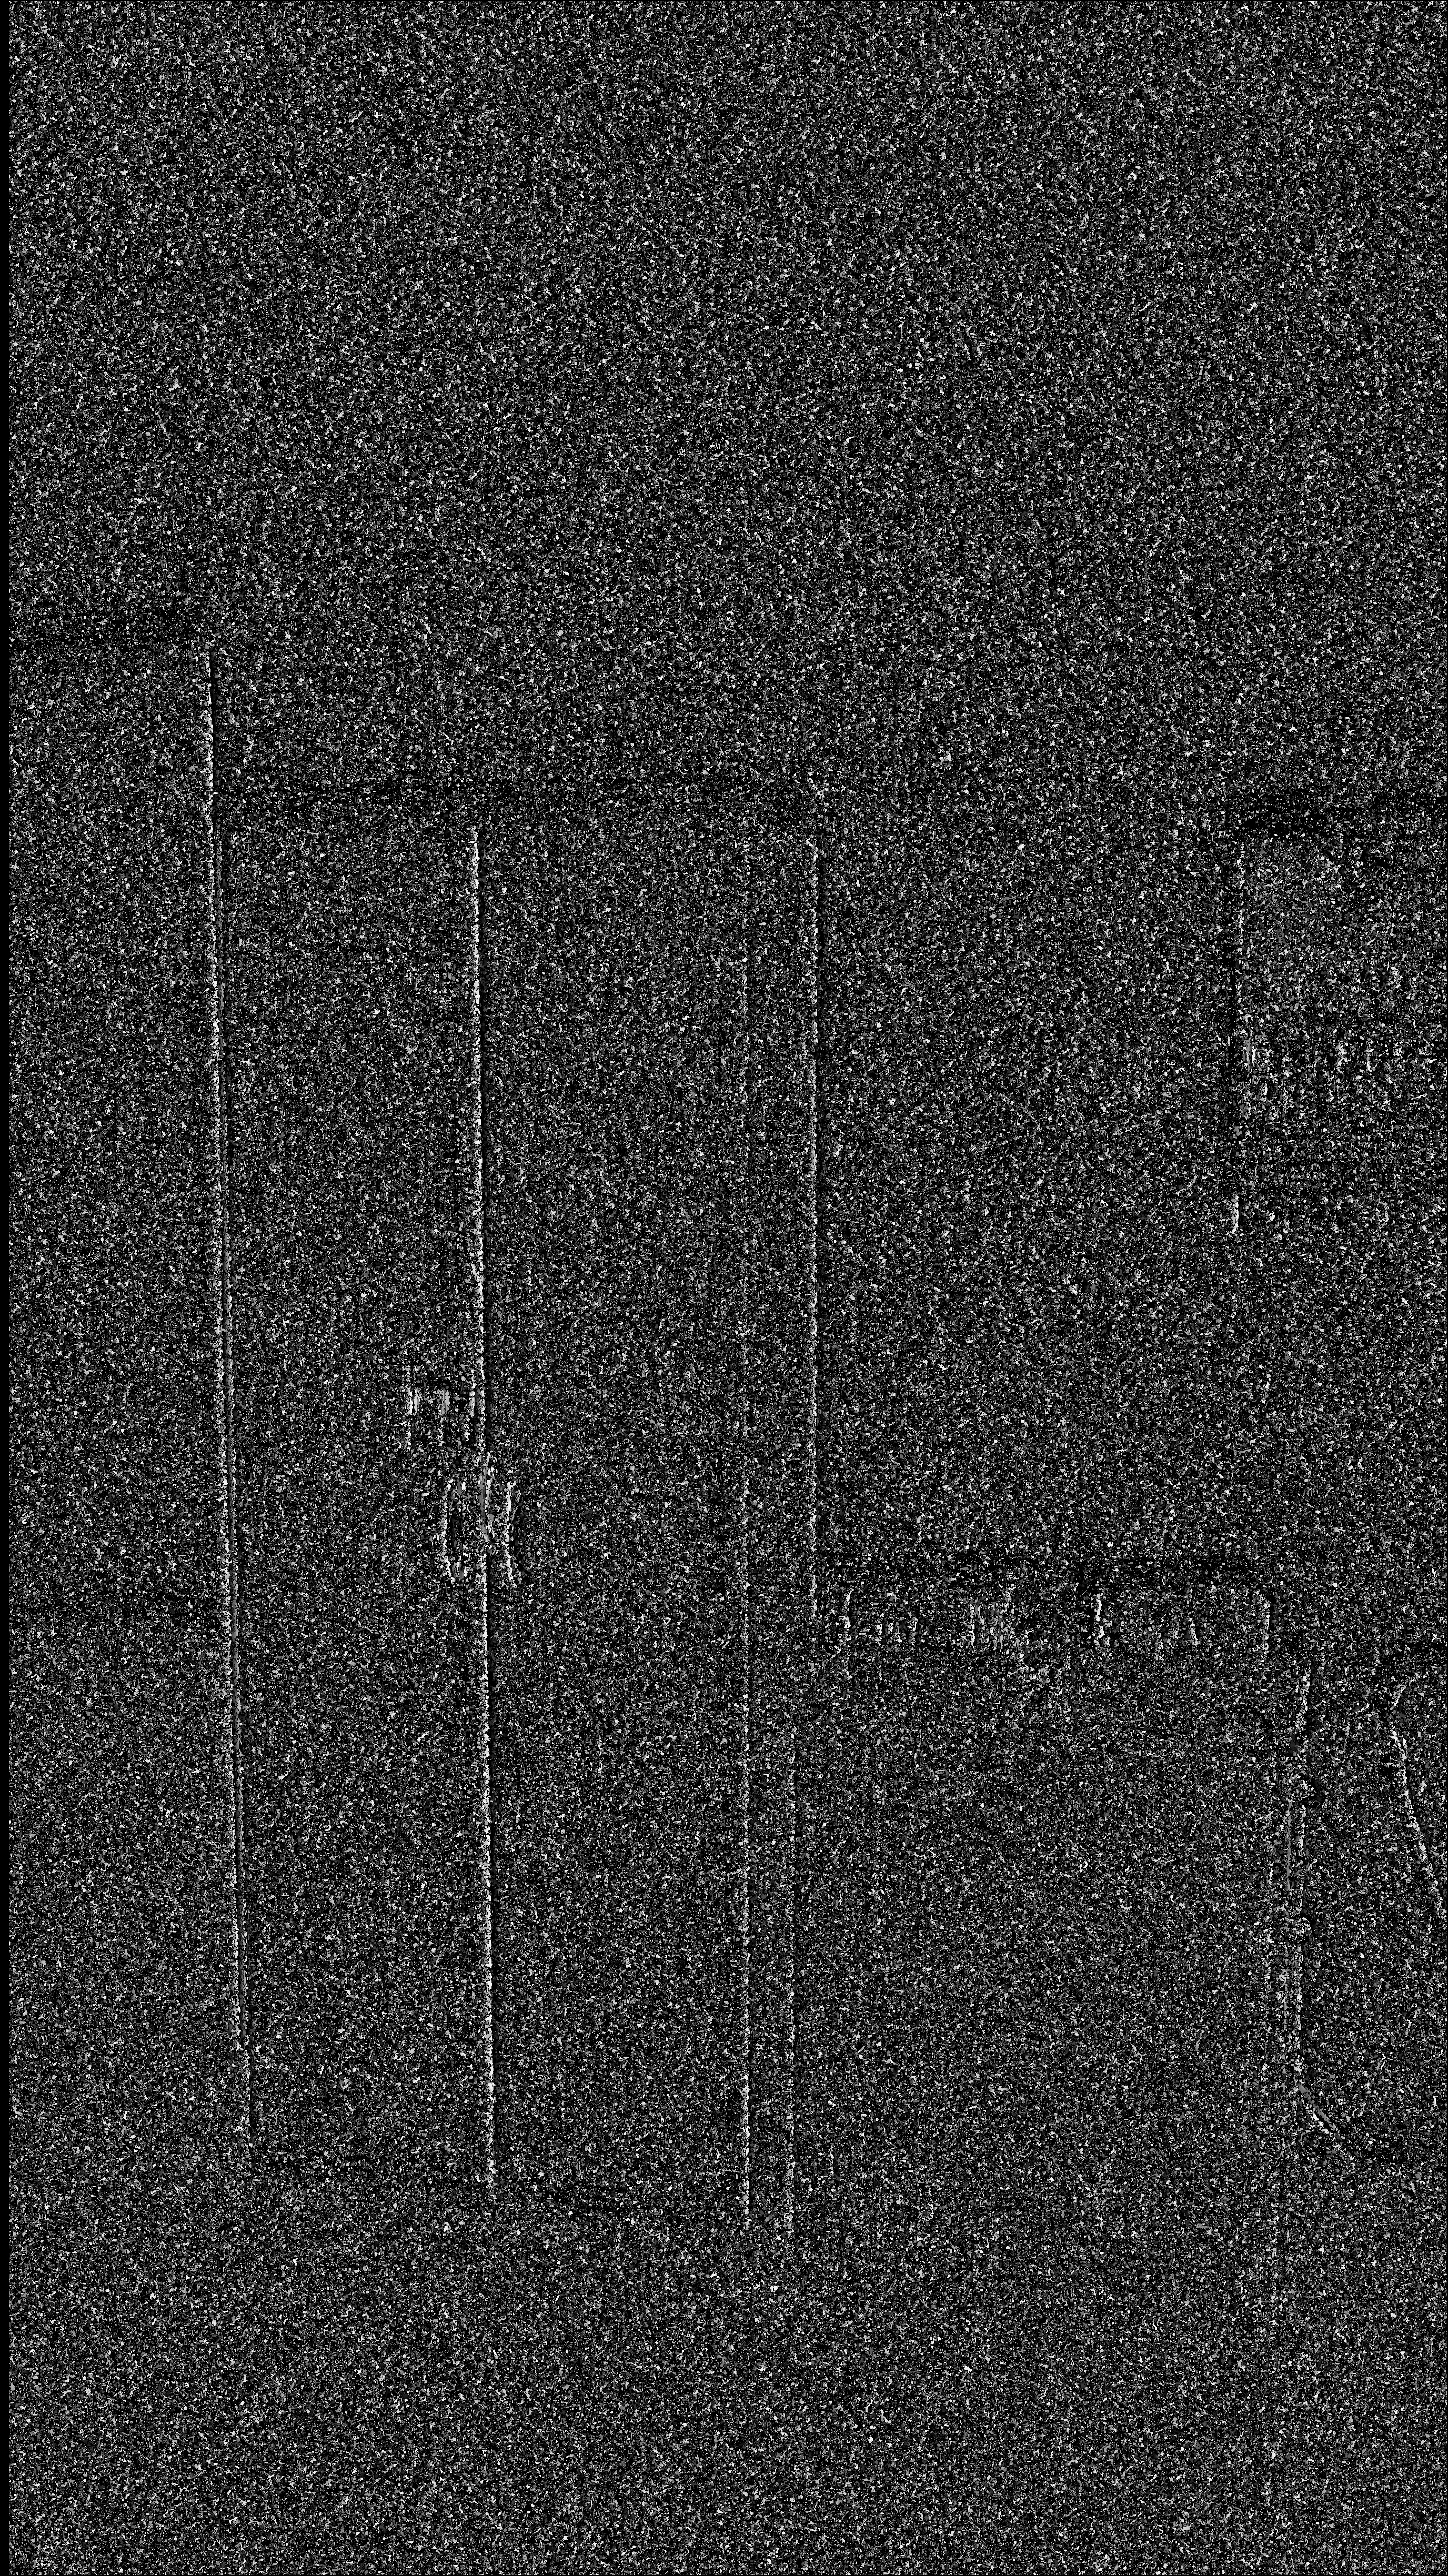
\includegraphics[width=\linewidth]{img/result}
	}
	\caption{Полученное изображение панорамы}
	\label{img:result}
\end{figure}